%%%% acra.tex

\typeout{ACRA Instructions for Authors}

% This is the instructions for authors for ACRA.
\documentclass{article}
\usepackage{acra}
% The file acra.sty is the style file for ACRA. 
% The file named.sty contains macros for named citations as produced 
% by named.bst.

% The preparation of these files was supported by Schlumberger Palo Alto
% Research, AT\&T Bell Laboratories, and Morgan Kaufmann Publishers.
% Shirley Jowell, of Morgan Kaufmann Publishers, and Peter F.
% Patel-Schneider, of AT\&T Bell Laboratories collaborated on their
% preparation. 

% These instructions can be modified and used in other conferences as long
% as credit to the authors and supporting agencies is retained, this notice
% is not changed, and further modification or reuse is not restricted.
% Neither Shirley Jowell nor Peter F. Patel-Schneider can be listed as
% contacts for providing assistance without their prior permission.

% To use for other conferences, change references to files and the
% conference appropriate and use other authors, contacts, publishers, and
% organizations.
% Also change the deadline and address for returning papers and the length and
% page charge instructions.
% Put where the files are available in the appropriate places.
\usepackage[pdftex]{graphicx}
%\usepackage{epstopdf}
% declare the path(s) where your graphic files are
\graphicspath{{./resources/}{./resources/tmp/}}
% and their extensions so you won't have to specify these with
% every instance of \includegraphics
\DeclareGraphicsExtensions{.pdf,.svg,.png}


\title{Use of AKKA Streams To Inform Forward Simulation in Robot Control}
\author{Peter Böhm\\ 
	ACME University, Australia\\ 
peter@nextlogic.biz}
%\author{Peter Böhm\textsuperscript{1} and Surya P. N. Singh\textsuperscript{2}\\ %\textsuperscript{1}ACME University, Australia\\ 
%	\textsuperscript{2}Robotics Design Lab, The University of Queensland, Australia\\
%	peter@nextlogic.biz, spns@uq.edu.au}

\begin{document}

\maketitle

\begin{abstract}
Computer simulations have become the standard for modeling of behavior of various natural systems. The more complex the model, the more sophisticated and more expansive hardware is required to run the simulation including multiple CPUs and GPUs. To achieve a realistic model, the simulation needs to be run on a high fidelity simulator like Microsoft's AirSim. Once the data has been generated, they need to be analyzed and the results visualized. The simulations often generate considerable amount of data about the simulated processes such as positions, velocities, rotations, collisions, environmental conditions, etc. During the simulation, these data need to be available to the solver for decision making calculations and possibly a progress visualizer. The data also need to be persisted for future analysis. When modeling interaction between multiple agents, the control and tracking of agents needs to be parallelized to allow for asynchronous operation and communication. The updates cannot happen in a single threaded control loop because that causes undesirable delays and move dependencies. The amount of work needed to create this supporting infrastructure is substantial and needs to be repeated or duplicated for every project. A middleware encapsulating these auxiliary services is presented.
\end{abstract}

\section{Introduction}

%\emph{Something about various uses of UAVs and importance of determination of the right strategy. Probably mention differential games as a theoretical framework and a couple of sentences about how it uses diff equations to describe the state. The simulation can be used to confirm the results in a realistic setting but also to train the agents, e.g. using RL. }
Over the last decade there has been an uptrend in the popularity of Unmanned Aerial Vehicles (UAVs.)

Training models offline using supervised learning is problematic as data is expensive to obtain and derived from inaccurate representations of the underlying aircraft dynamics. An alternative to supervised learning for creating offline models is known as reinforcement learning (RL). In RL an agent is given a reward for every action it makes in an environment with the objective to maximize the rewards over time. Using RL it is possible to develop optimal control policies for a UAV without making any assumptions about the aircraft dynamics. Recent work has shown RL to be effective for UAV autopilots, providing adequate path tracking. \cite{rlForUAVs}

Typically, the reinforcement learning works with a simulator. The simulator provides observations, and then a learning algorithm has a policy which chooses an action. The simulator then processes the action and returns a reward. When this is applied to the real-world, however, there are many differences. The observation that comes from the real-world differs from the simulator in various ways. In simulator it is easy to control environment and say step forward one step please. But in the real-world, typically the environment controls you. In simulator, state is the fundamental information necessary in order to make a decision. But in the real world there are some very complex observations which may have much more information than it is necessary to make a decision. If you have a megapixel camera, you don't need all the pixels settings as a state. \cite{real-world-bandits}

%\emph{Couple of sentences about simulators, how they are important because the realistically model the environment and it's one less very messy thing to worry about. Briefly discuss some of the available sims, their strengths and weaknesses?}
For the RL models to be effective in the real-world, the agent needs to be trained in a real-world like environment. To provide a realistic real-world model is a non-trivial task. The agents need to rely on inputs that are also available in real-world such as sensors, LIDAR, camera depth view, segmentation view or the FPV (first-person view). In this case it may be important to model real-world complex objects such as trees, roads, lakes, electric poles and houses along with rendering that includes finer details such as soft shadows, specular reflections, diffused inter-reflections and so on. \cite{shah2018airsim}

This kind of environment is provided by high fidelity simulators, such as AirSim, Carla or Gazeebo. This text describes integration with AirSim. AirSim is a simulator for drones, cars and more, built on Unreal Engine. It is open-source, cross platform, and supports hardware-in-loop with popular flight controllers such as PX4 for physically and visually realistic simulations. It is developed as an Unreal plugin that can simply be dropped into any Unreal environment. \cite{shah2018airsim}
\emph{maybe an image with the 3 views}

%\emph{More details about AirSim - something like the conclusion from the MS paper. How it provides actual location but also sensors}


\section{Background}
%\emph{Example of a naive python program working with AirSim - sending instructions and receiving state updates. First show figure with only the 2 processes and then add on everything else necessary and show how it becomes entangled. Then split it up into the solver, persistence, visualization, etc. all connected by the middleware. }
\begin{figure}
	\centering
	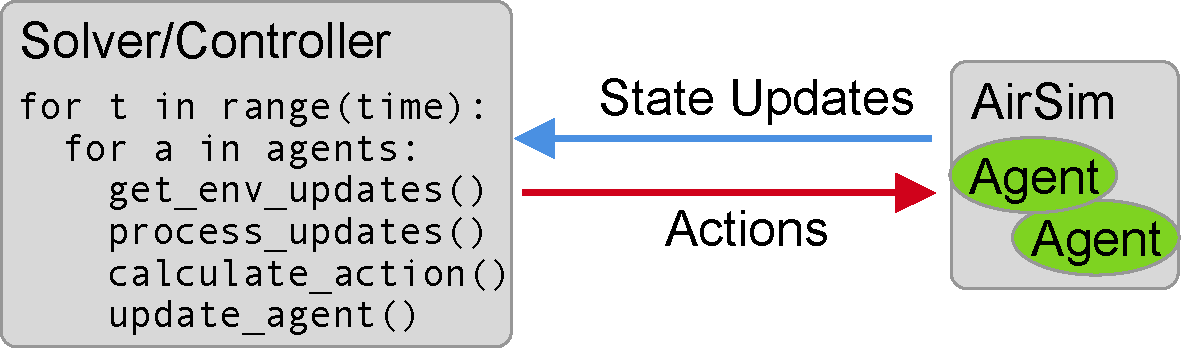
\includegraphics[width=8.31cm]{naive-solver}
	\caption{Example of a simple solver interacting with the simulator.}\label{fig:naive-solver}
\end{figure}

Figure \ref{fig:naive-solver} shows a simple solver/controller interacting with the simulator using a simple time loop. This is a common design for a classic RL episode, however, there are several limitations with respect to the high fidelity simulator. 
\begin{itemize}
	\item Concurrency - in realistic settings, the agents make decisions and move independently and concurrently, not sequentially. Each agent may also have different limitations, such as measurement delay, accuracy, etc.
	\item Time step - because the time in the simulation flows independently, and calculations for each step may take different amount of time (during which the agents are moving), it is necessary to set the time in time units (e.g. 60s, 5min, etc.) rather than number of steps.
	\item Settings - agents require a number of settings such as identification in the simulator, action strategy, top velocity, turning radius, pilot delay, etc. If these are hard coded, it becomes difficult to reproduce the experiments and may require recompilation after every run.
	\item Visualization - while the simulator may provide various observer camera settings, it may not be possible to see all actors if they are not close to each other and the simulator will not display the trajectories taken by the agents needed for more precise visualization.
	\item Persistence - the simulator requires a high end machine with GPU, however, once the data has been generated and recorded, it can be visualized and analyzed on a commodity hardware.
	\item Support for different solvers - 
\end{itemize}




\subsection{Concurrency and Timestamp} 
Because the simulator provides a realistic world-like model, it also needs to be interacted with in a realistic way. One of the main differences when compared to the low or mid fidelity simulators, such as OpenAI Gym, is absence of a turn by turn event loop.
E.g., the Mountain Car problem in OpenAI Gym (Figure \ref{fig:mountain-car}) simulates effects gravity and inertia, however, after every action taken by the agent, the time is suspended. The agent can take as long as it needs to calculate the next action. At that point, the time and physics starts moving again and the car moves without any loss of inertia or speed.
\begin{figure}
	\centering
	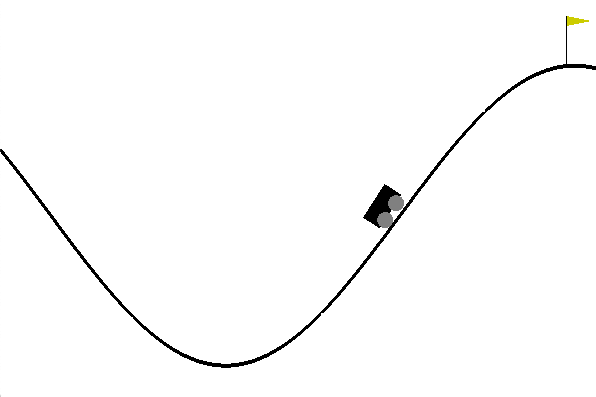
\includegraphics[width=7cm]{mountain-car}
	\caption{Mountain car problem in the OpenAI Gym. The car can be suspended and resumed without any loss of momentum.}\label{fig:mountain-car}
\end{figure}

In a high fidelity simulator, the situation is different. The agents receive commands, however, the time and the underlying physics do not stop in between the commands. As such it is important that the tasks that can run in parallel, such as location tracking and controlling of the agent are parallelized. This is especially important in multi-agent simulations, where the forced sequence and the delay between actions of the agents can have material impact on the progress and results of the simulation. The tasks that can run in parallel include sampling the environment state (e.g. location updates, sensor measurements, image from the camera, etc.), processing this input (e.g. calculation of relative distances, LIDAR points analysis), calculation of the new direction/speed and sending of the commands to the agents. If the turnaround time for a single agent is about 0.5s (which is reasonable even in real life situations), with two agents moving sequentially, the total delay will be around 1s. At speeds of 10m/s, this would significantly affect maneuverability of the agents. In purser/evader simulation, this could easily make the difference between escape and capture (see Figure \ref{fig:single-vs-multi-thread}).

\begin{figure}
	\centering
	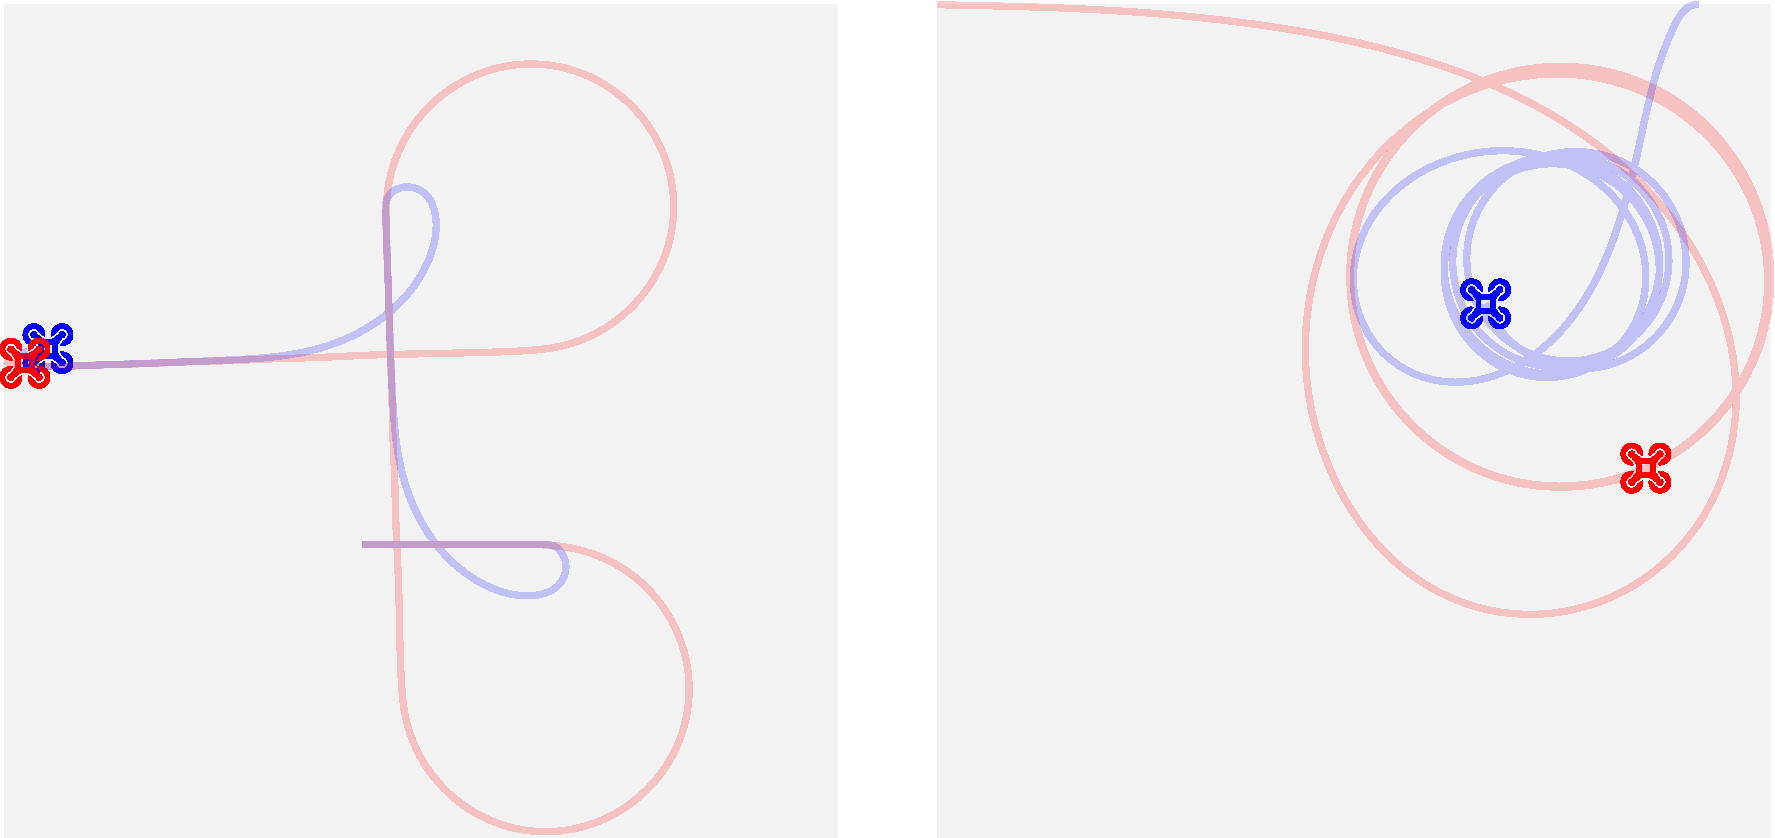
\includegraphics[width=8.3cm]{single-vs-multi-thread}
	\caption{Both images show the algorithm pursue/evade algorithm. The left was run in a single threaded event loop and the right was parallelized using Akka Actors.}\label{fig:single-vs-multi-thread}
\end{figure}


\section{Programming Model}
As shown, the two main differences of working with high fidelity simulators: data streams and concurrency.

\subsection{Reactive Streams}
High fidelity simulators, just like real-world implementations, generate large amount of data that needs to be processed in near real-time. Each agent can generate multiple streams (e.g. location updates, camera feed, LIDAR feed, etc.) and streams from multiple agents may need to combined (e.g. in synchronized movement of multiple vehicles). Each stream may need multiple transformations (e.g. deserialization, conversion, calculations, etc.) and those transformations may need to be parallelized to increase throughput.
Reactive Streams is an initiative to provide a standard for asynchronous stream processing with non-blocking back pressure. This encompasses efforts aimed at runtime environments (JVM and JavaScript) as well as network protocols. \cite{reactive-manifesto} 

In a system without back pressure, if the subscriber is slower than the publisher, then eventually the stream will stop - either because one of the parties runs out of memory and one of its buffers overflows or because the implementation can detect this situation but cannot  stop sending or accepting data until the situation is resolved (if it can be resolved at all). Although the latter scenario is somewhat more positive than the former, blocking back pressure (the capability of a system to detect when it must slow down and to do so by blocking) brings with it all of the disadvantages of a blocking system, which occupies resources such as thread and memory usage. \cite{reactive-web-apps}

Besides technical reasons, there is also additional motivation for the reactive stream. They provide a DSL (Domain Specific Language) \cite{dsl-book} to define the stream transformation graphs in a expressive way. 

\begin{figure}
	\centering
	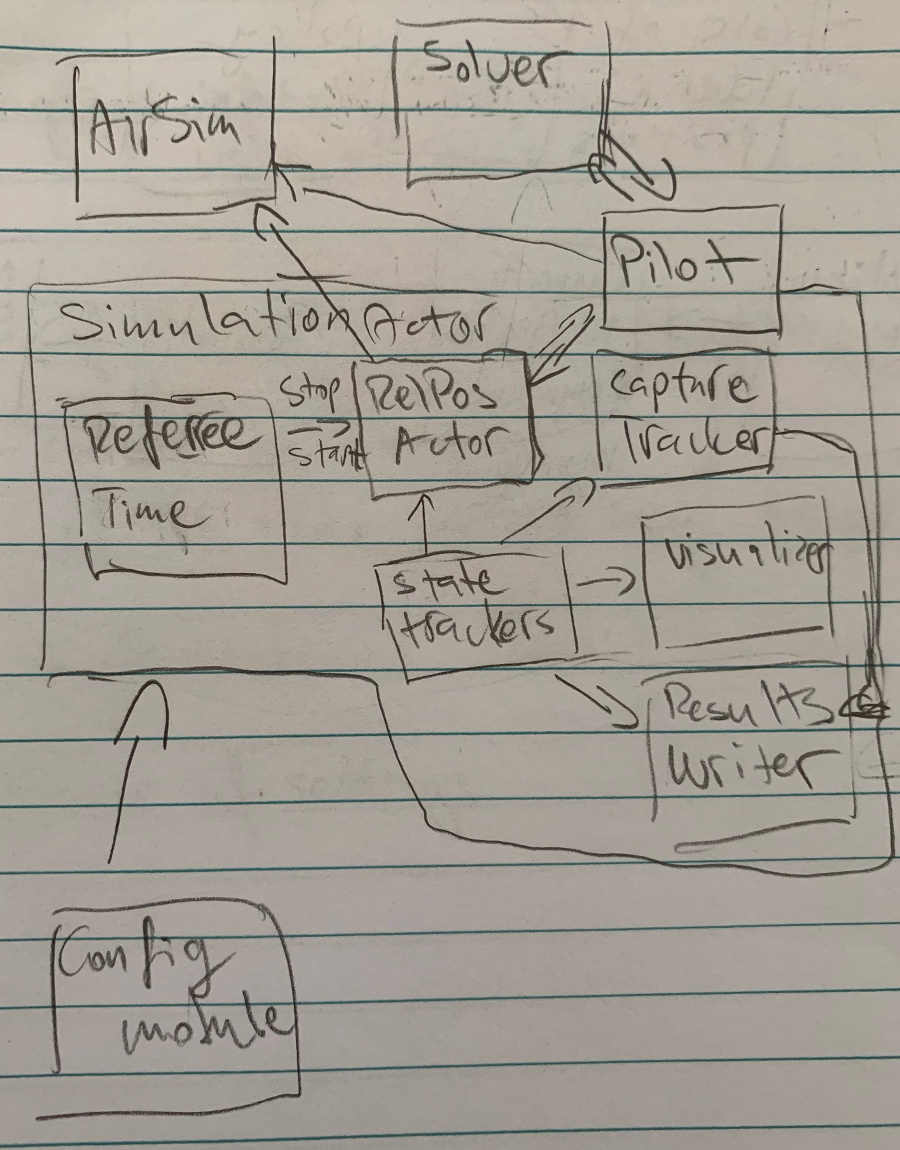
\includegraphics[width=6.0cm]{before-flow}
	\caption{System design without streams.}\label{fig:before-stream}
\end{figure}

On a micro level, the simulation can be seen as a set of steps (query the environment, evaluate the result, decide the next action, send the action to the environment, etc.), however, on the macro level it can be viewed as data flow. There is some data flowing out of the environment (location updates, camera stream, etc.) and some data flowing back in (steering directions). Without the data flow, the system resembles the Figure \ref{fig:before-stream}. The components interact freely to receive the data they need to do their job. If the components are encapsulated as \verb|Actor|s to allow for parallel processing of messages, this represents a workable solution. With growing number of sensor outputs and varying requirements of the solver inputs, however, it becomes difficult to maintain and extend.


\subsection{Actor Model}
Something about concurrency issues and how actor model addresses them?
Need for new programming model (something like Akka Docs intro).
Routing



\subsection{Message Broker}
For situation where the solver cannot be implemented in the same program (e.g. because it is implemented in a different programming language) or on the same machine (e.g. because it requires extra resources such as GPU), it is necessary to implement remote messaging.
 
One way is to use some kind of RPC (Remote Procedure Call) solution. There are several available: AirSim uses MessagePack RPC (Remote Procedure Call), Google uses gRPC for its services, and there are several others. Another option is to use a message broker. The difference is that while RPC calls the remote service directly, with message broker, the services publish and consume messages via the message broker.

Kafka was developed to collect and distribute massive messages for distributed systems. It is a high-throughput distributed messaging system. Kafka can always keep stable performance even if it processes millions of messages per second. \cite{wang2015kafka}

Figure \ref{fig:after-kafka} shows how such communication works. The raw (or pre-processed) data is published to Kafka (e.g. one topic for location updates, one topic for LIDAR, etc.) and consumed by services that process these data. The results are then published to a different topic. This simplifies dependencies between services, reduces data loss when a service crashes, provides a simplicity of one "API" for communication.



\begin{figure}
	\centering
	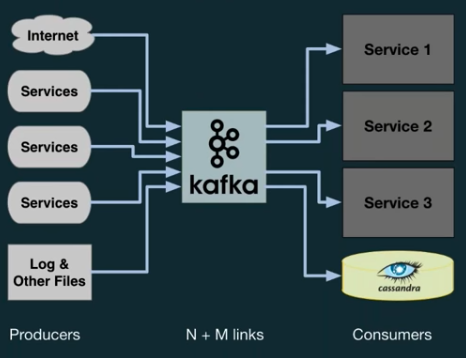
\includegraphics[width=5cm]{after-kafka}
	\caption{Message broker handles  .}\label{fig:after-kafka}
\end{figure}

\subsection{Results Visualization}
A good visualization tool should not only visualize the final outcome as an animation but also expose the data behind every step. It should allow to change the presentation speed, pause, rewind, etc.  Scalable Vector Graphics (SVG), a web-native format provides an easy way to create animation from the generated data. Unlike the more common raster format, vector images are defined in terms of 2D points connected by lines and curves to form polygons and other shapes. \cite{basicShapes}

The animation of the objects is done using simple JavaScript and DOM (Document Object Model) manipulation. \cite{masteringSVG} SVG object have transform attribute that accepts arguments for 5 transformations (translate, scale, rotate, skewX and skewY). Translate and scale are most relevant for the simulations. Translate accepts 2 parameters \verb|tx| and \verb|ty| and moves objects to new coordinates calculated as \verb|initialX - tx| and \verb|initialY - ty|. 

The scale is used to scale the trajectories up or down to fit the screen. Because the view shows both scalable objects (e.g. trajectories) and non-scalable objects (e.g. text, icons, etc.), it is better to pre-scale the location coordinates using the axis aligned bounding rectangle before using them to position the objects and draw trajectories.



\section{Implementation}

Each simulation runs within its own parent actor \verb|SimulationRunnerActor|. Based on the settings provided, this actor sets up all the auxiliary services (e.g. time keeper, visualizer, capture detector) as child actors. It also sets up an Akka Stream for each agent and each tracked sensor and location updates. The simulation is terminated either by the \verb|TimeKeeperActor| when the time has completed or if some termination event is detected (e.g. capture detected by \verb|CaptureDetectorActor|). At this point a kill switch is activated on the streams and the \verb|SimulationRunnerActor| receives a poison pill which stops all the child actors and shuts down the simulation.

Running the entire simulation within the context of a single parent actor allows multiple simulations to run in parallel.

\subsection{Settings}
Just like in AirSim, the amount of available configuration options is too high to be supplied as command line arguments or to be hard-coded before each run. A better option is to use a configuration file but, unlike with AirSim, this configuration should be editable at runtime without the need to restart the program after each change.
This could be a separate UI component like in Figure \ref{fig:config-module}. After each run the user can update the parameters and run another simulation. The configuration module generates an updated config file and passes it to the simulation runner that uses it to create the simulation.

Another option is a grid-search controller, that takes some initial configuration and accepts value ranges for the selected parameters. Based on this input, it generates multiple settings files and runs a simulation for each of them.

\begin{figure}
	\centering
	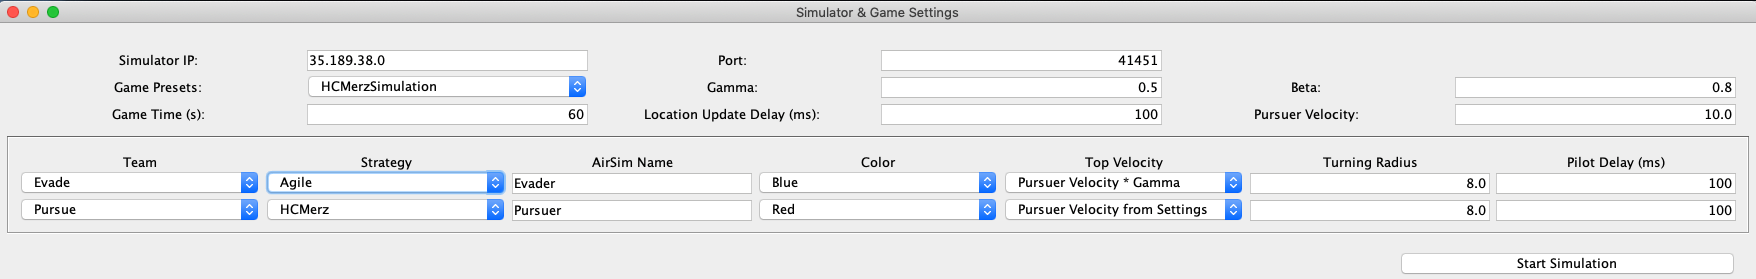
\includegraphics[width=8.6cm]{config-module}
	\caption{UI for configuration module.}\label{fig:config-module}
\end{figure}

\begin{figure}
	\centering
	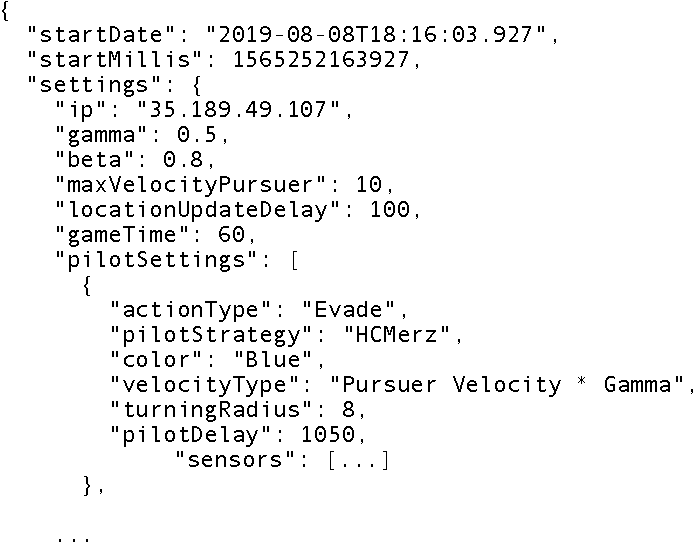
\includegraphics[width=8.6cm]{settings}
	\caption{Sample of the config file in JSON format.}\label{fig:settings-format}
\end{figure}


\subsection{Communication with AirSim}

AirSim uses MessagePack \cite{messagepack} for communication. Some of the methods calls are non-blocking (e.g. methods for controlling the vehicles such as \verb|moveByVelocityZ|), however, methods returning vehicle's state, camera feed, LIDAR feed are blocking. The return time of the blocking methods is especially important when using a cloud GPU to run AirSim. Depending on the network connection and type (e.g. VPN), the latency of \verb|getMultirotorState| (a method that returns position, orientation, velocity and acceleration of the vehicle) can be as high as 100ms.


\begin{figure}
	\centering
	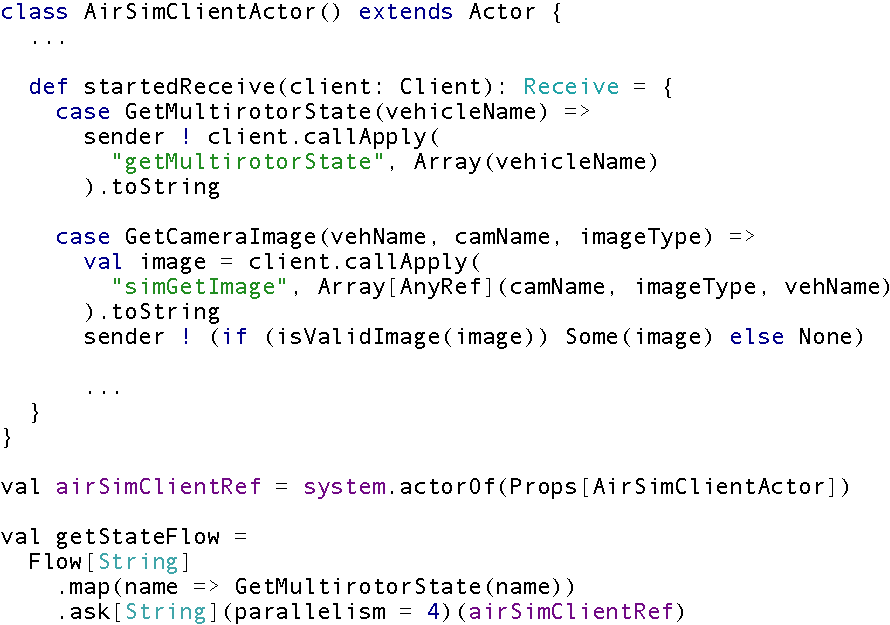
\includegraphics[width=8.6cm]{air-sim-client}
	\caption{Flow transforming vehicle name to multi-rotor state string.}\label{fig:air-sim-client}
\end{figure}


Because multiple components need to interact with AirSim and the interaction is stateless (the only state is the open connection, but each connection can handle any commands from any component), it is a good use-case for Akka routing. Akka Router creates a pool of actors and each of them opens a connection at the start of the simulation. If a component (e.g. position tracker) requires location update, it passes a message to the router. The router then routes the message to the actor. Once the actor receives a response from AirSim, it returns it to the component in the form of message. Because most of the components are Akka Streams and not actors, this call is encapsulated in a \verb|Flow| using the ask pattern. 

A simplified code is shown in Figure \ref{fig:air-sim-client}. \verb|AirSimClientActor| receives messages such as \verb|GetMultirotorState| or \verb|GetCameraImage|, interacts with the AirSim and returns the result to the sender of the message. Flow \verb|getStateFlow| uses \verb|ask| pattern to interact with the actor. Parallelism argument is related to back pressure. It allows these calls to be parallelized (e.g. if some of the responses take longer to process than the query interval).

\subsection{Akka Streams}
Figure \ref{fig:with-flow} shows implementation using Akka Streams. Each data flow is encapsulated in the stream. The incoming data is received by a merge/broadcast component that provides a publisher/subscriber functionality. The downstream components subscribe for the input they need (this is transparent to the data producers). Solvers are a special category, because they do not behave as sinks, they behave as flows (i.e. transformations). Solvers transform the input into the output in the form of actions and these actions and then routed through the \verb|AirSimClientActor| back to the AirSim.

\begin{figure}
	\centering
	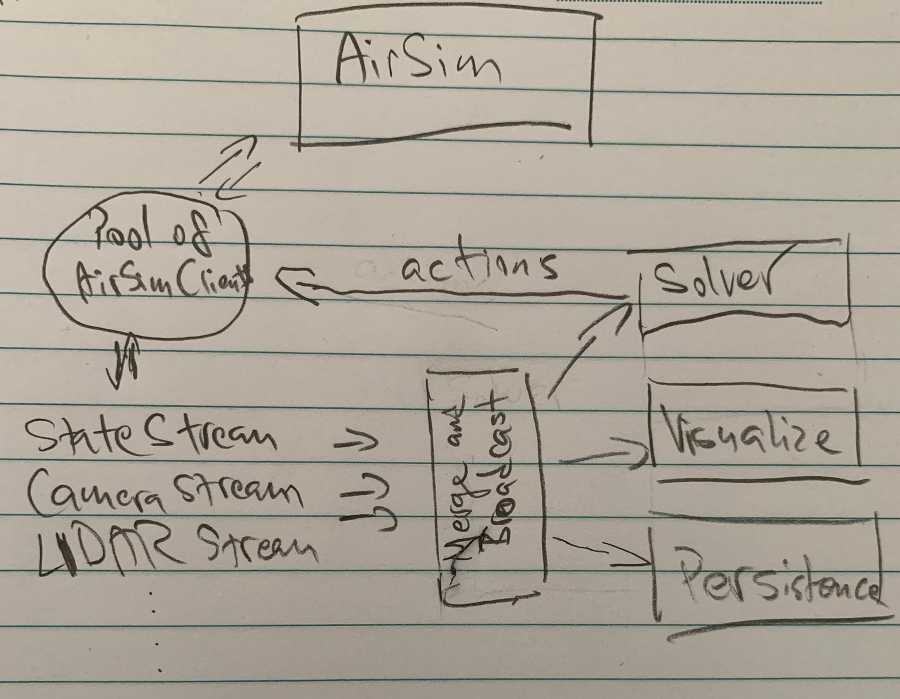
\includegraphics[height=5cm]{with-flow}
	\caption{Implementation using Akka Streams.}\label{fig:with-flow}
\end{figure}

% instead show code handling 2 streams and generating a response?
\begin{figure}
	\centering
	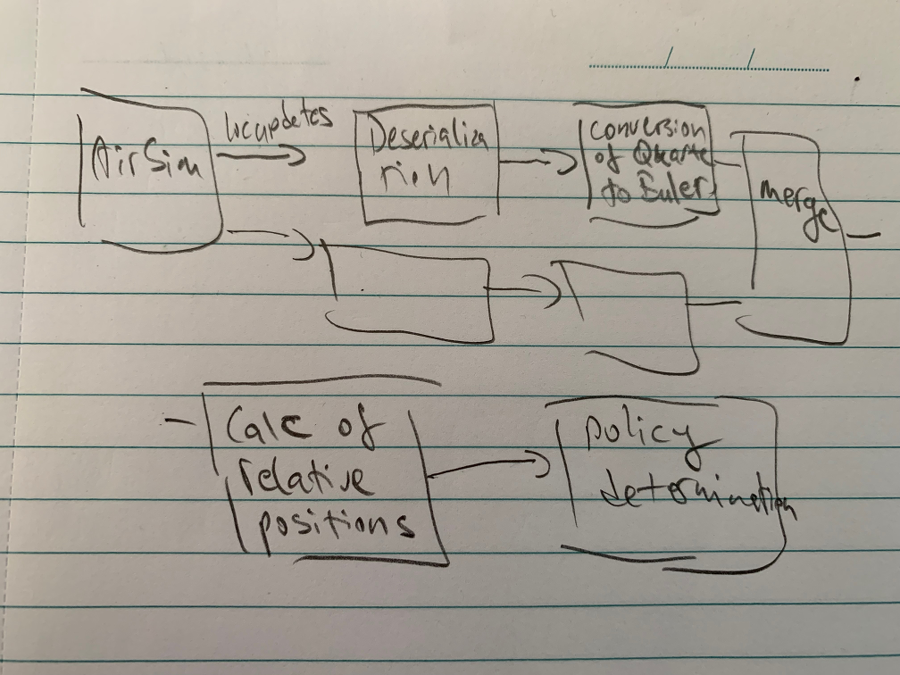
\includegraphics[width=6cm]{flow-in-sketch}
	\caption{Graph handling location updates stream. Data is received from AirSim, deserialized, converted and fed into the solver that determines the next action.}\label{fig:flow-in}
\end{figure}

%
%\begin{figure}
%	\centering
%	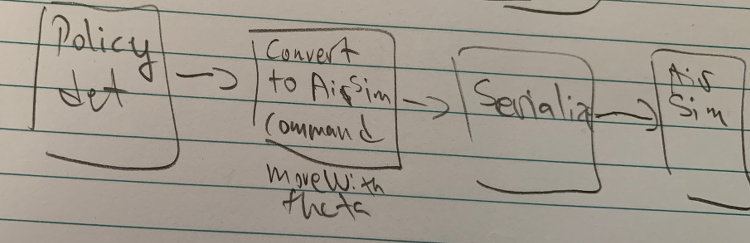
\includegraphics[width=6cm]{flow-out-sketch}
%	\caption{Graph streaming the selected action back to AirSim. The solver returns steering %angle theta that needs to be converted to AirSim command moveByVelocityZ, serialized and sent %to AirSim. }\label{fig:flow-out}
%\end{figure}

\subsection{Kafka}
Implementation using Kafka is somewhat similar to the above solution but instead of built-in solver, the streams are terminated in Kafka. Figure \ref{fig:kafka-sink} shows such implementation. These messages are then received by the solver (or any other program), e.g. in Python using \verb|KafkaConsumer|. The solver generates action and this action is then posted back to Kafka on a different topic. Back in the middleware the actions are consumed and using the \verb|AirSimClientActor| routed back to AirSim.

\begin{figure}
	\centering
	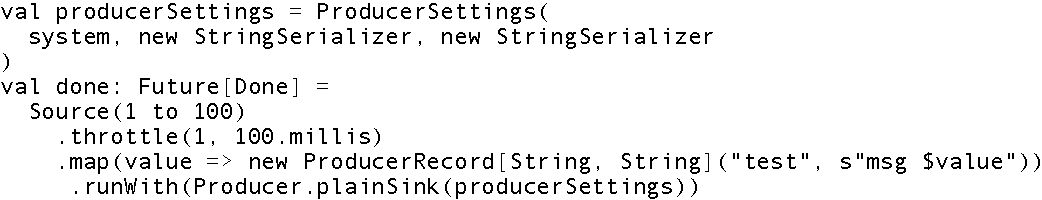
\includegraphics[width=8.3cm]{kafka-sink}
	\caption{Serializing Akka Stream to Kafka.}\label{fig:kafka-sink}
\end{figure}

\subsection{Visualizer}

The visualizer is implemented using SVG. The persisted data streams from location trackers are used to create animation. Each vehicle is represented as a separate shape. The visualizer iterates over the location data and translates the shapes to their respective positions. Each new location is added to the polylines representing the trajectories of each agent. The visualizer also displays additional information useful for debugging such as the current timestamp, position of each agent, distance between the agents and the capture count.
It also provides controls to manage animation speed, movement on the time line, etc.

\begin{figure}
	\centering
	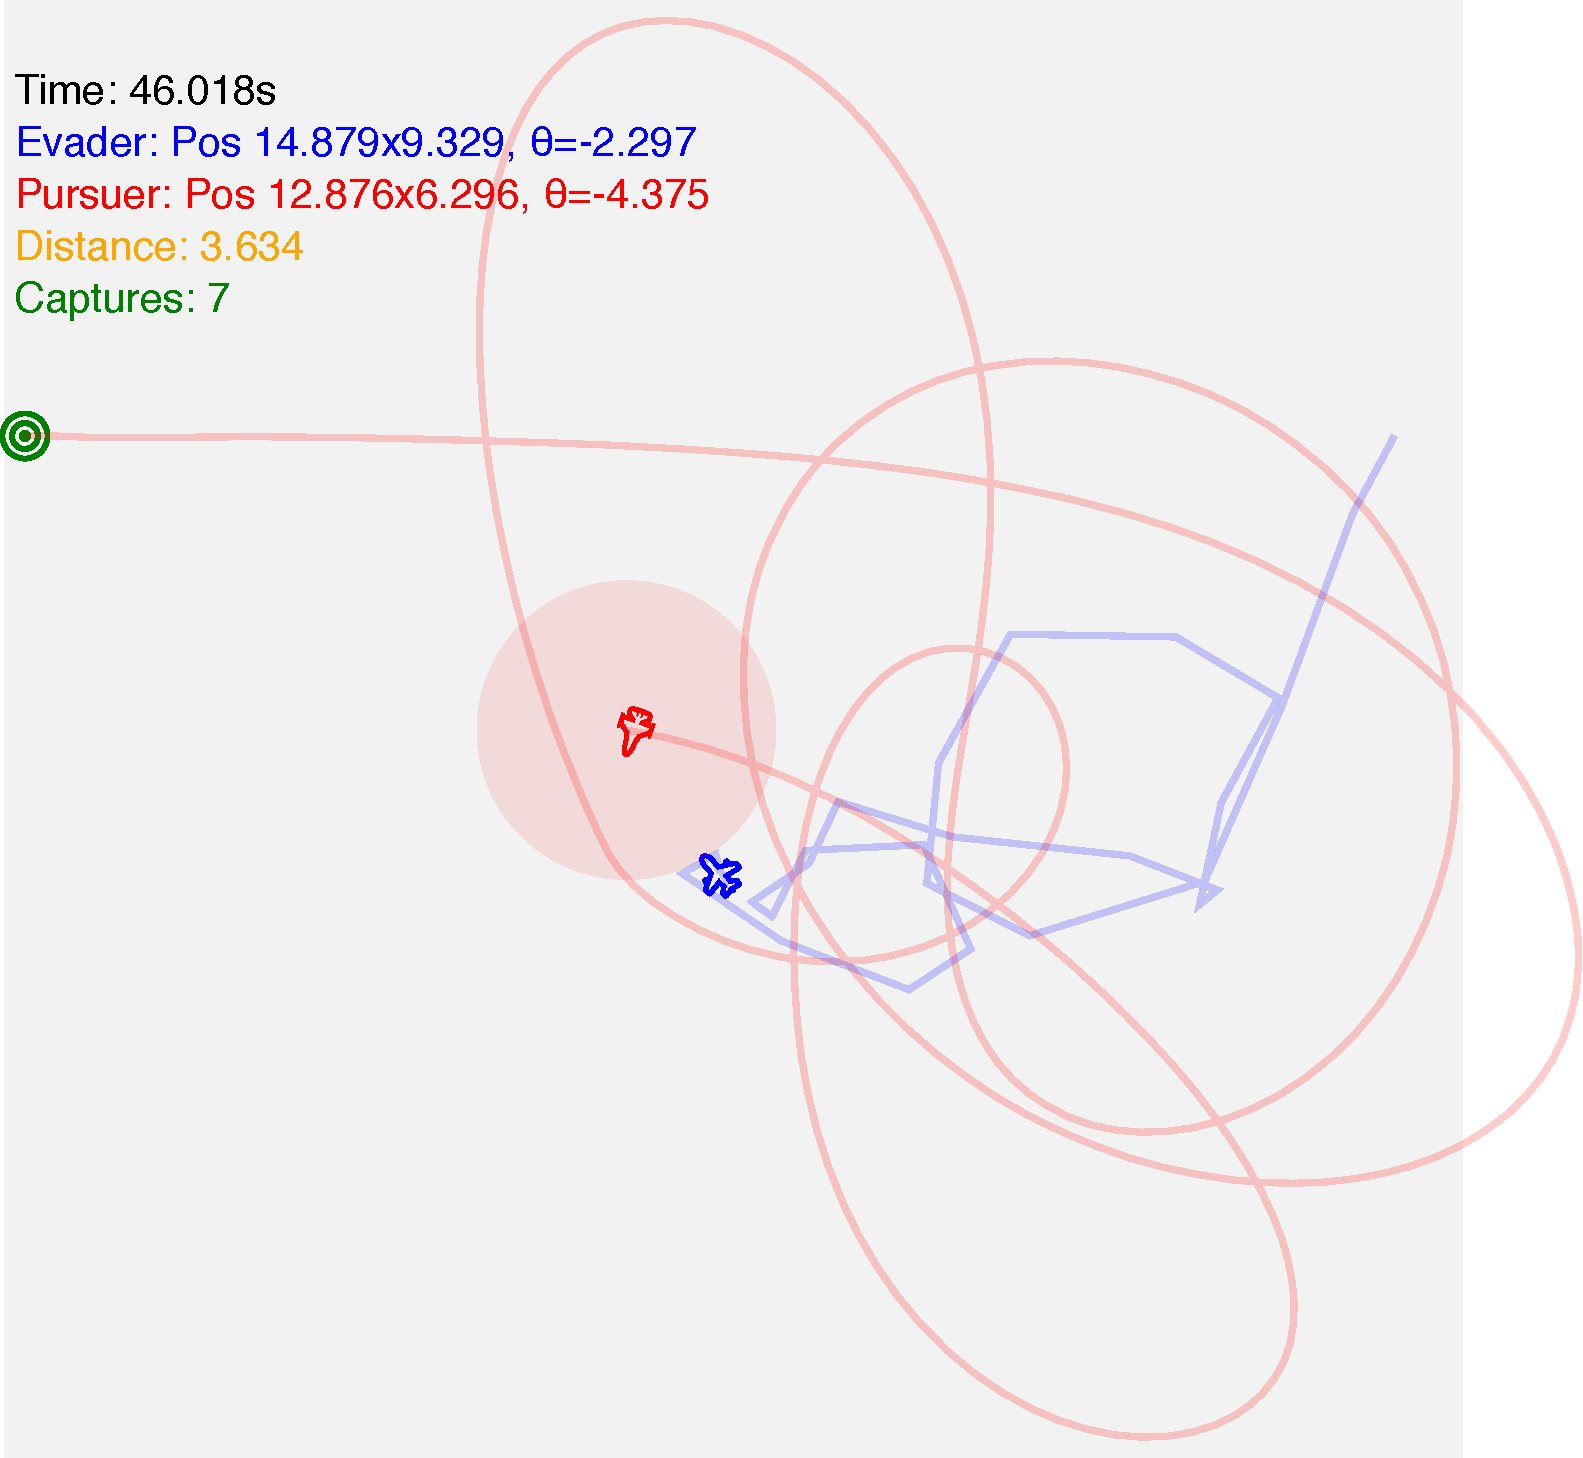
\includegraphics[width=8.3cm]{visualizer}
	\caption{Snapshot of the visualizer view.}\label{fig:visualizer}
\end{figure}


\subsection{Persistence}

The main body of the text immediately follows the abstract. 
Use 10-point type in a clear, readable font with 1-point leading (10 on
11).  For reasons of uniformity, use Computer Modern font if possible.  If
Computer Modern is unavailable, Times Roman is preferred.

Indent when starting a new paragraph, except after major headings.


\section{Conclusions}

\section*{Acknowledgments}
The preparation of these instructions and the LaTEX and BibTEX files that implement them was supported by Schlumberger Palo Alto Research, AT\&T Bell Laboratories, and Morgan Kaufmann Publishers.


%% This section was initially prepared using BibTeX.  The .bbl file was
%% placed here later
%\bibliography{publications}
%\bibliographystyle{named}
%% The file named.bst is a bibliography style file for BibTeX 0.99c
\bibliographystyle{named}
\bibliography{bibfile}



\end{document}

